\chapter{Conductivity Modelling}
\label{chap:conductivity}
The conductivity of the ionosphere is the primary factor in the ionospheric continuity equation coefficients as proposed by~\citet{goodman1995} (Equation~\ref{eqn:continuity_eqn}). As discussed in Section~\ref{sec:height_integrated_conductivities}, the charged particle density is a driving factor in the variation of height integrated conductivities. The variation in the levels of charged particles in the ionosphere occurs due to both incident extreme ultraviolet (EUV) rays from the sun causing ionization in the ionosphere and auroral precipitation along the magnetic field lines~\citep{cousins2015}. Both of these are available through multiple empirical models, see \citet{moen1993,cousins2015, hardy1987}. This application has been designed to be agnostic to the choice of conductivity model to allow new models to be added and swapped without recompilation. In this section the conductance models that are currently implemented will be discussed along with plans for future conductivity model support, and the structure of this model's conductivity modeling.
\section{EUV Conductivities}
\label{sec:euv_conductivity}
The first main source of conductivity within the ionosphere is the ionization of particles in the ionosphere due to incident extreme ultraviolet radiation. This is the primary contribution to conductivity in the low latitude regions of the Earth. Even at high latitudes, when the auroral contribution is low the Hall and Pedersen conductivities are primarily driven by variations in solar EUV radiation~\citep{moen1993}.
\subsection{Moen Brekke EUV Conductivity Model}
The EUV conductivity model that has been implemented currently is the empirical model produced by \citet{moen1993}. This model provides an empirical formula for the EUV driven Hall and Pedersen conductivity as a function of F10.7 solar flux level $S_a$ and solar zenith angle $\chi$. This data is produced from EISCAT incoherent scatter data of the electron density profiles.
\begin{equation}
	\Sigma_H(\chi, S_a) = S_a^{0.53}(0.81\cos\chi + 0.54\cos^{1/2}\chi)
\end{equation}
\begin{equation}
	\Sigma_P(\chi, S_a) = S_a^{0.49}(0.34\cos\chi + 0.93\cos^{1/2}\chi)
\end{equation}
Figure~\ref{fig:euvPedersonVsSeason} displays EUV conductivity contributions to the height integrated Pedersen conductivity over three different dates. Seasonal variation can result in different distributions of conductivity through the ionosphere. This can have large effects on the final solution to Equation~\ref{eqn:continuity_eqn} as this can greatly influence behaviour on the poles. This is explored further in Chapter~\ref{chap:results}. This seasonal variation is provided by differing solar zenith angle distributions at different times of the year. The process of calculating the solar zenith angle is discussed in Section~\ref{sec:conductivity_implementation}, and the F10.7 solar flux levels are configurable through the YAML application configuration file.
\begin{figure}[H]
	\centering
	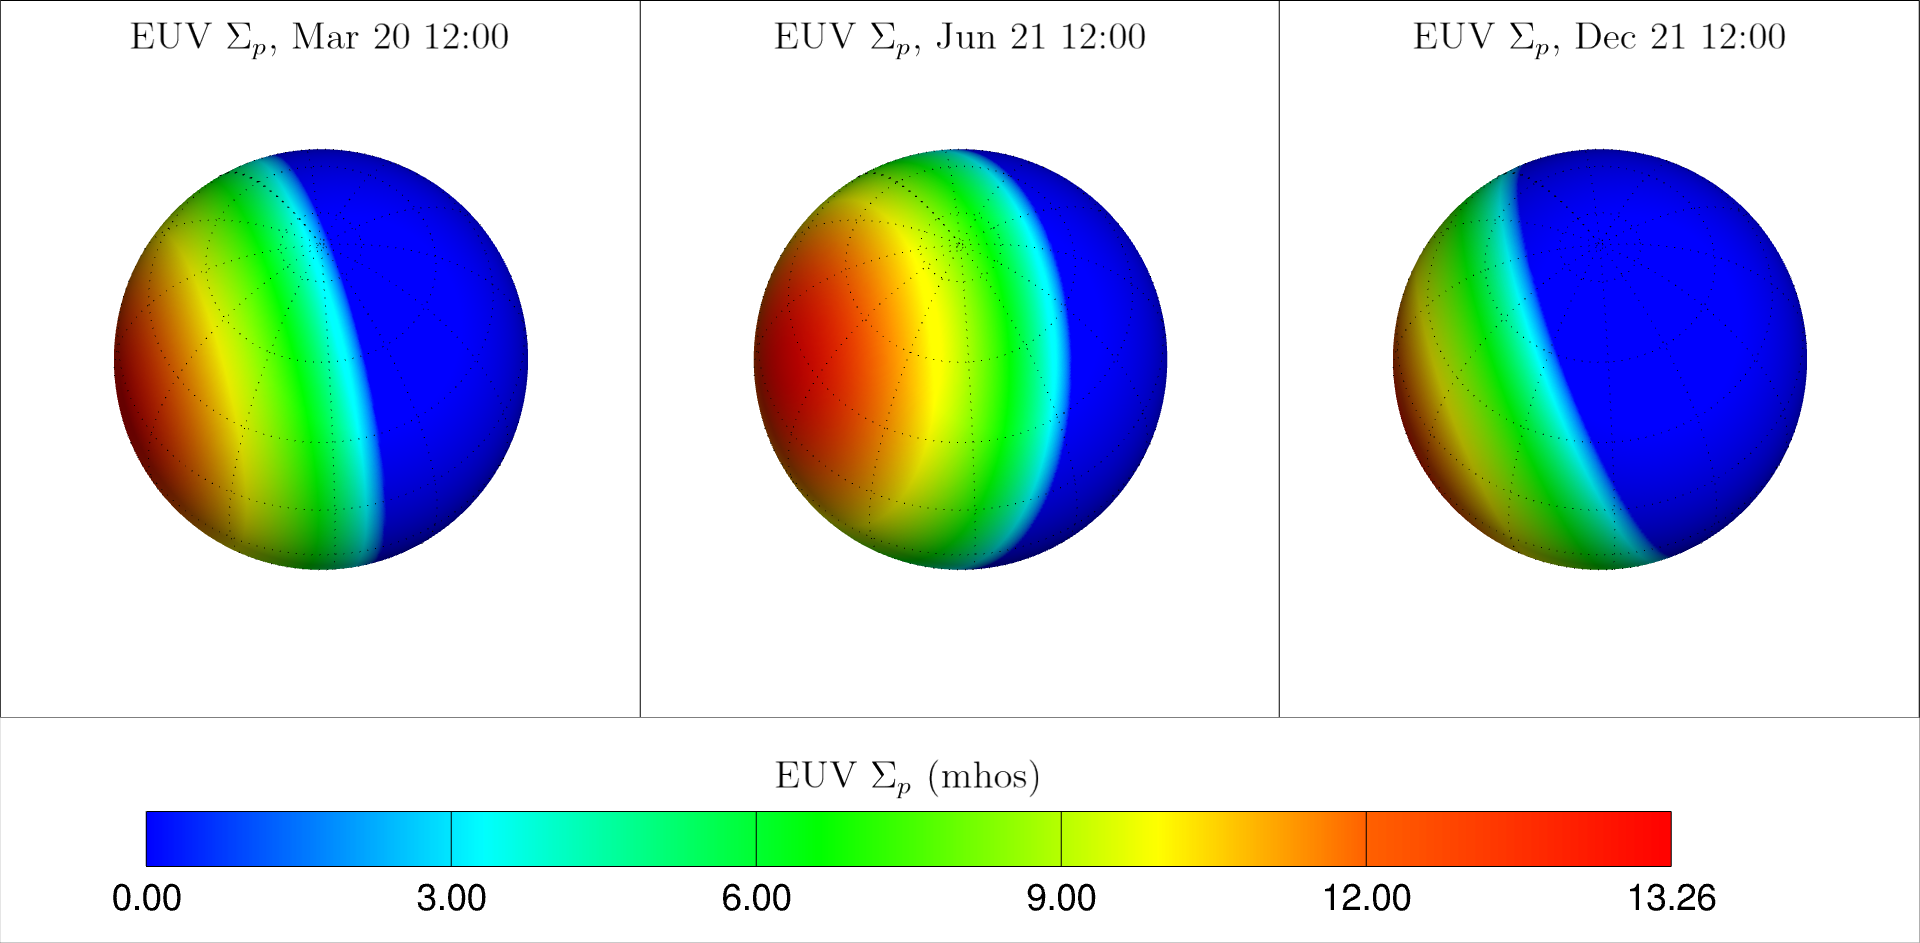
\includegraphics[width=\textwidth]{figures/euvlPedersonVsSeason.png}
	\caption{EUV-driven Pedersen conductance $\Sigma_p$ (mhos) for equinox (Mar 20), summer (Jun 21), and winter (Dec 21) at 12:00 UT, showing the seasonal variation of EUV conductivity.}
	\label{fig:euvPedersonVsSeason}
\end{figure}
\section{Auroral Conductivities}
The second main source of the ionospheric conductivity is through electrons introduced to the ionosphere through auroral precipitation. The strong magnetosphere-ionosphere coupling along field lines drives particle precipitation. Electrons precipitate into the ionosphere along magnetic field lines~\citep{hardy1987}, increasing the conductivity levels as discussed in Section~\ref{sec:height_integrated_conductivities}. Due to the structure of the Earth's magnetic field, this precipitation primarily occurs at high latitudes~\citep{hardy1987}. Considering that the high latitude region acts as the primary interface for magnetosphere-ionosphere coupling, the accuracy of the conductivities in this region is of utmost importance to the accuracy of the model~\citep{hardy1987}.

\subsection{Hardy Conductivity Model}
The auroral conductivity model that is currently implemented is the empirical model produced by \citet{hardy1987}. This paper used particle flux measurements from the SSJ/3 detectors aboard the DMSP F2 and F4 satellites and the CRL-251 detector aboard P78-1 to model the global auroral precipitation, following the conductivity derivation approach of~\citet{spiro1982}. The Hardy model models the auroral Hall and Pedersen conductivities using the Epstein transition function (Equation~\ref{eq:epstein_transition}).
\begin{equation}
	e(h) = r + S_1(h - h_0) + (S_2 - S_1) \cdot \ln\left\{
	\frac{1 - S_1/(S_2 e^{-(h-h_0)})}{1 - (S_1/S_2)}\right\}
	\label{eq:epstein_transition}
\end{equation}
The four values in this function are provided by the paper as sixth order Fourier series coefficients. These coefficients are binned by the magnetic activity index $K_p$ and the coefficients are then computed using a Fourier series with magnetic local time as the parameter as shown in Equation~\ref{eq:fourier_series}. These Fourier series provide the peak latitude ($h_0$), and the amplitude and slope parameters ($r$, $S_1$, $S_2$). The magnetic latitude is determined by the corresponding position on the grid.
\begin{equation}
	a(T) = \sum_{n=0}^{6}\left\{C_n^a \cos\left[\frac{n\pi T}{12}\right]
	+ S_n^a \sin\left[\frac{n\pi T}{12}\right]\right\}
	\label{eq:fourier_series}
\end{equation}
This provides a function for the Hall and Pedersen conductivities that is a function of the magnetic local time, magnetic activity index and magnetic latitude. The calculation of the magnetic local time required additional models to be implemented within the application. The magnetic activity index ($K_p$) is configurable through the YAML configuration file. The calculation of magnetic local time and the application structure is discussed further in Section~\ref{sec:conductivity_implementation}.

\begin{figure}[H]
	\centering
	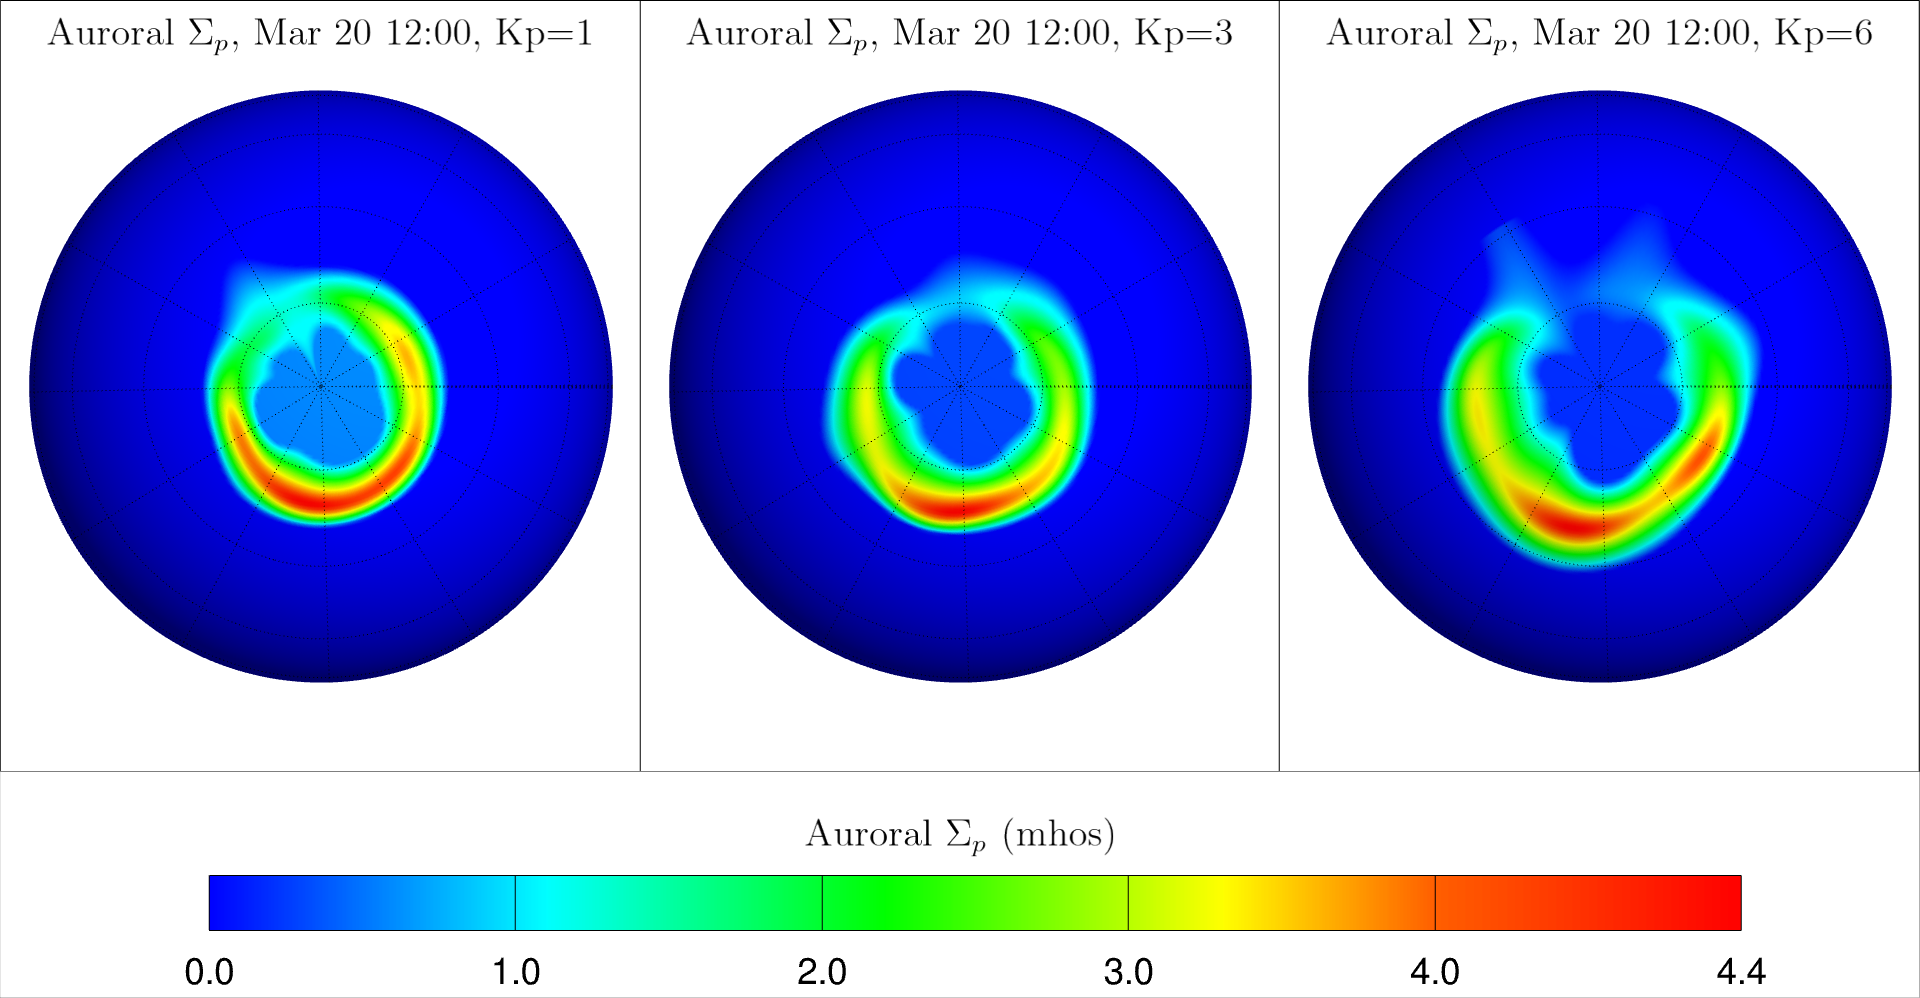
\includegraphics[width=\textwidth]{figures/auroralPedersonVsKp.png}
	\caption{Auroral Pedersen conductance $\Sigma_p$ (mhos) for $K_p = 1$, $3$, and $6$ on (Mar 20, 12:00), showing the expansion of the auroral conductance with increasing geomagnetic activity.}
	\label{fig:auroralPedersonVsKp}
\end{figure}
Figure~\ref{fig:auroralPedersonVsKp} displays three sample conductivity distributions for the height integrated Pedersen conductivity from the Hardy model over three different geomagnetic activity levels. The expansion of the auroral oval at high $K_p$ values can be seen clearly.

\section{Conductivity Combination}
To combine the two sources of conductivity, \citet{wallis1981} describes an approximation for determining the total conductivity from the auroral and EUV conductivities. This involves taking the root mean squared summation of the two conductivities as shown in Equation~\ref{eq:cond_combination}.
\begin{equation}
	\Sigma_{i, total} = \sqrt{\Sigma_{i, auroral}^2 + \Sigma_{i, EUV}^2}
	\label{eq:cond_combination}
\end{equation}
This was the method that was chosen for combining the contributions from each of the conductivity models. \citet{wallis1981} found the error of this approach to be $\sim$ 15\% and $\sim$ 7\% for $\Sigma_H$ and $\Sigma_P$ respectively when $\Sigma_{i,auroral} \approx \Sigma_{i,EUV}$. Therefore, this is not a good approximation for regions where both the auroral and EUV conductivities are contributing similarly. Due to the differing latitudes between the peak EUV-driven conductivity and the auroral conductivity, this error will by mainly focused on a band of mid-latitude points where the values are similar. Figure~\ref{fig:totalConductivity} shows the total conductivity computed within the simulation both with auroral and EUV contributions for both the Hall and Pedersen conductances. This is an example case of a low error combination due to the distributions of the EUV contribution and the auroral contribution being relatively distinct.
\begin{figure}[H]
	\centering
	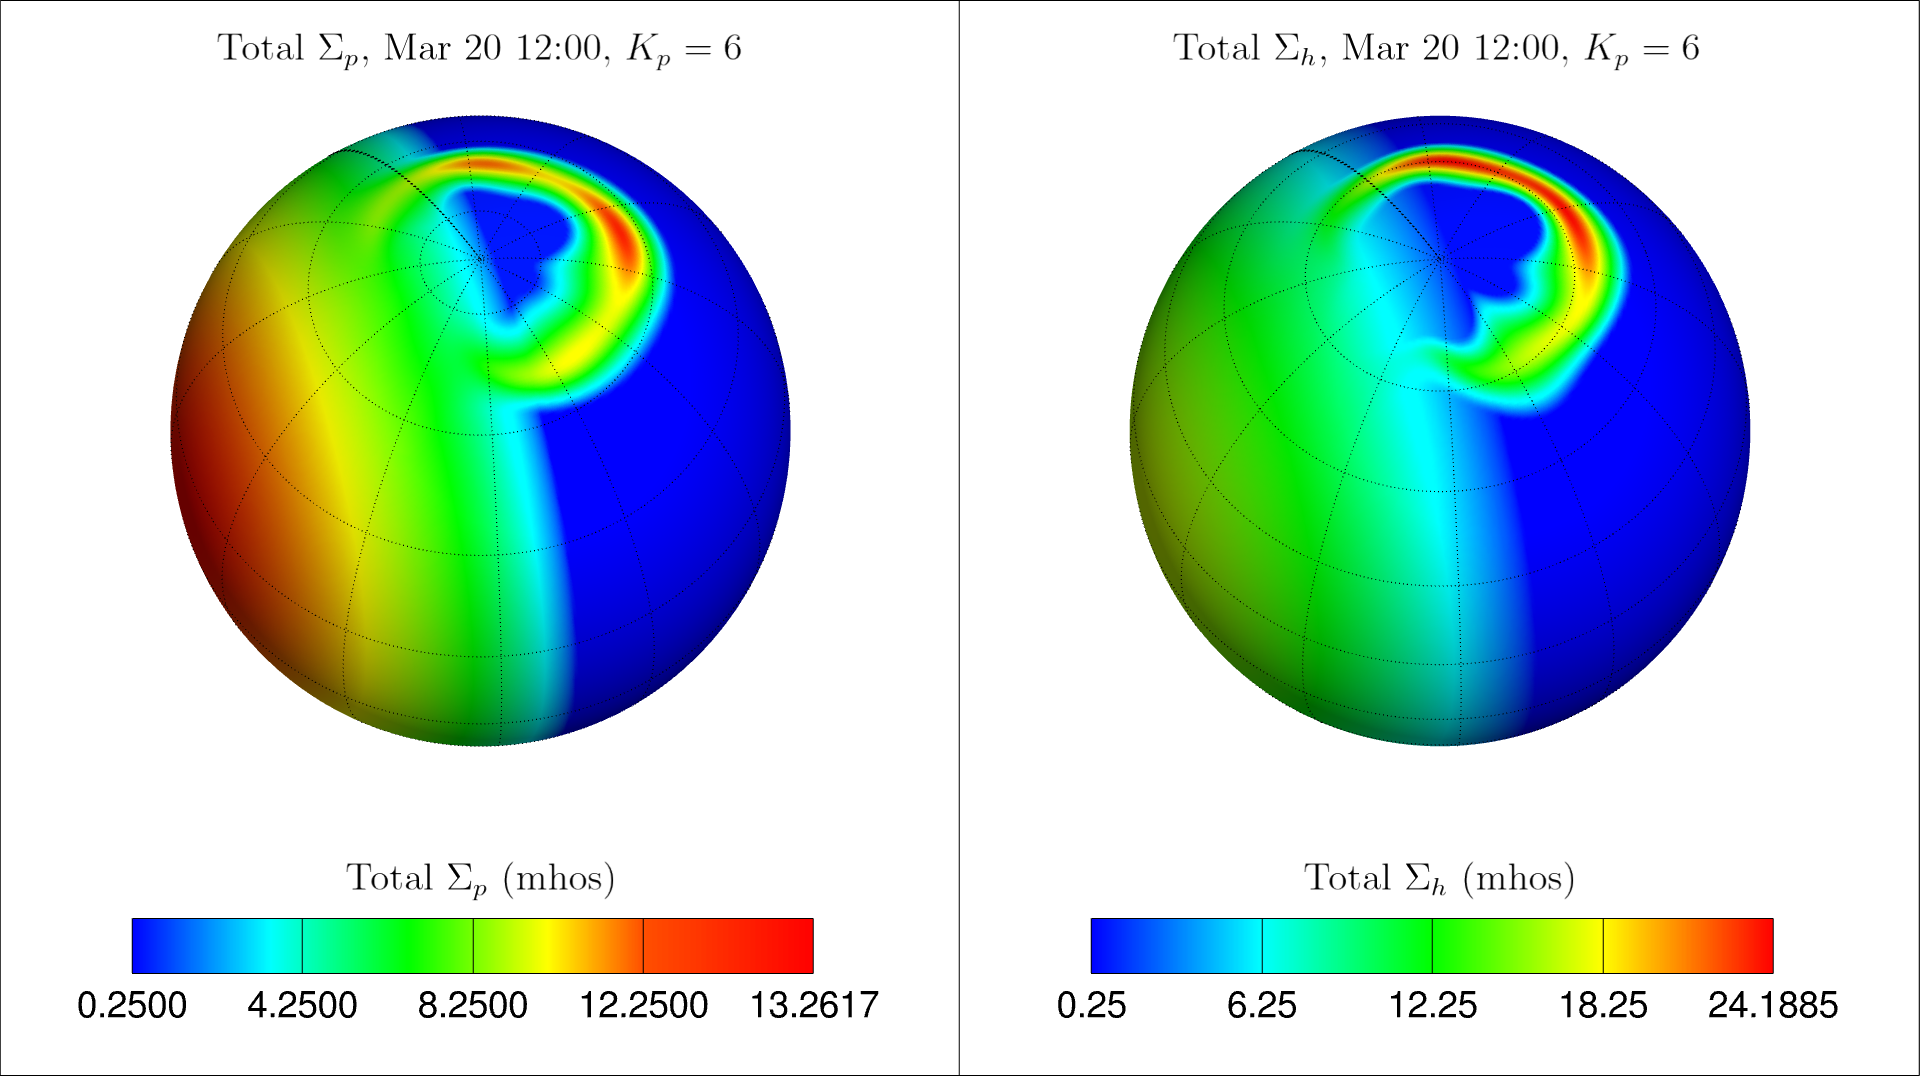
\includegraphics[width=\textwidth]{figures/totalConductivity.png}
	\caption{Total Pedersen ($\Sigma_p$) and Hall ($\Sigma_h$) conductances (mhos) for $K_p = 6$ at equinox (Mar 20, 12:00), combining EUV and auroral contributions.}
	\label{fig:totalConductivity}
\end{figure}

\section{Implementation}
\label{sec:conductivity_implementation}
To facilitate extensibility, the application was designed to be as configurable as possible without recompilation. Even though only one model is implemented so far within this system, the conductivity models implement an abstract interface and are injected through a factory function. This allows for the ability to hot-swap the conductivity models without recompilation when new ones are added. Additionally, new conductivity models can be built in the application by implementing the existing interface. Figure~\ref{diag:conductivity_diagram} shows the structure of the conductivity models that are currently implemented.
\begin{figure}[H]
	\centering
	\includestandalone[width=0.7\textwidth]{diagrams/ConductivityDiagram}
	\caption{Data flow diagram showing the structure of the conductivity model. Conductance tensor at the bottom is fed into the solver portion of the application through an abstract interface. The full system diagram is available in Figure~\ref{diag:full_flow2}.}
	\label{diag:conductivity_diagram}
\end{figure}
The auroral and EUV conductivity models required computation of the magnetic local time and solar zenith angle respectively. To achieve this, some additional small models were included in the application as seen in Figure~\ref{diag:conductivity_diagram}. These provided the ability to convert between magnetic dipole coordinates and geographic coordinates and to compute the solar zenith angle and magnetic local time.

The solar zenith angle is determined for all points on the grid using the third method described in~\citet{grena2012}. This provides the ability to compute the solar zenith angle for all points on the globe from a date and time configurable within a YAML configuration file. The solar zenith angle model required geographical coordinates, while the main coordinate system used in the ionosphere model is magnetic dipole coordinates. To make this conversion, the geographic to dipole conversion matrix described in~\citet{laundal2017} was included to create a rotational matrix that allowed for conversion between the two coordinate systems. By using the latest IGRF magnetic field coefficients available in \citet{igrf2024}, the dipole rotational matrix was then constructed. This matrix was used for coordinate transformations when required. The dipole matrix is interpolated between five year epochs using the provided parameters in~\citep{igrf2024}.

Figure~\ref{fig:mltAlignment} displays the magnetic local time as calculated in the ionosphere model. The magnetic local time is calculated by solving for the subsolar point (the point at which the sun's incidence is perpendicular to the Earth) and using that to calculate the relative times for all points on the grid.
\begin{figure}[H]
	\centering
	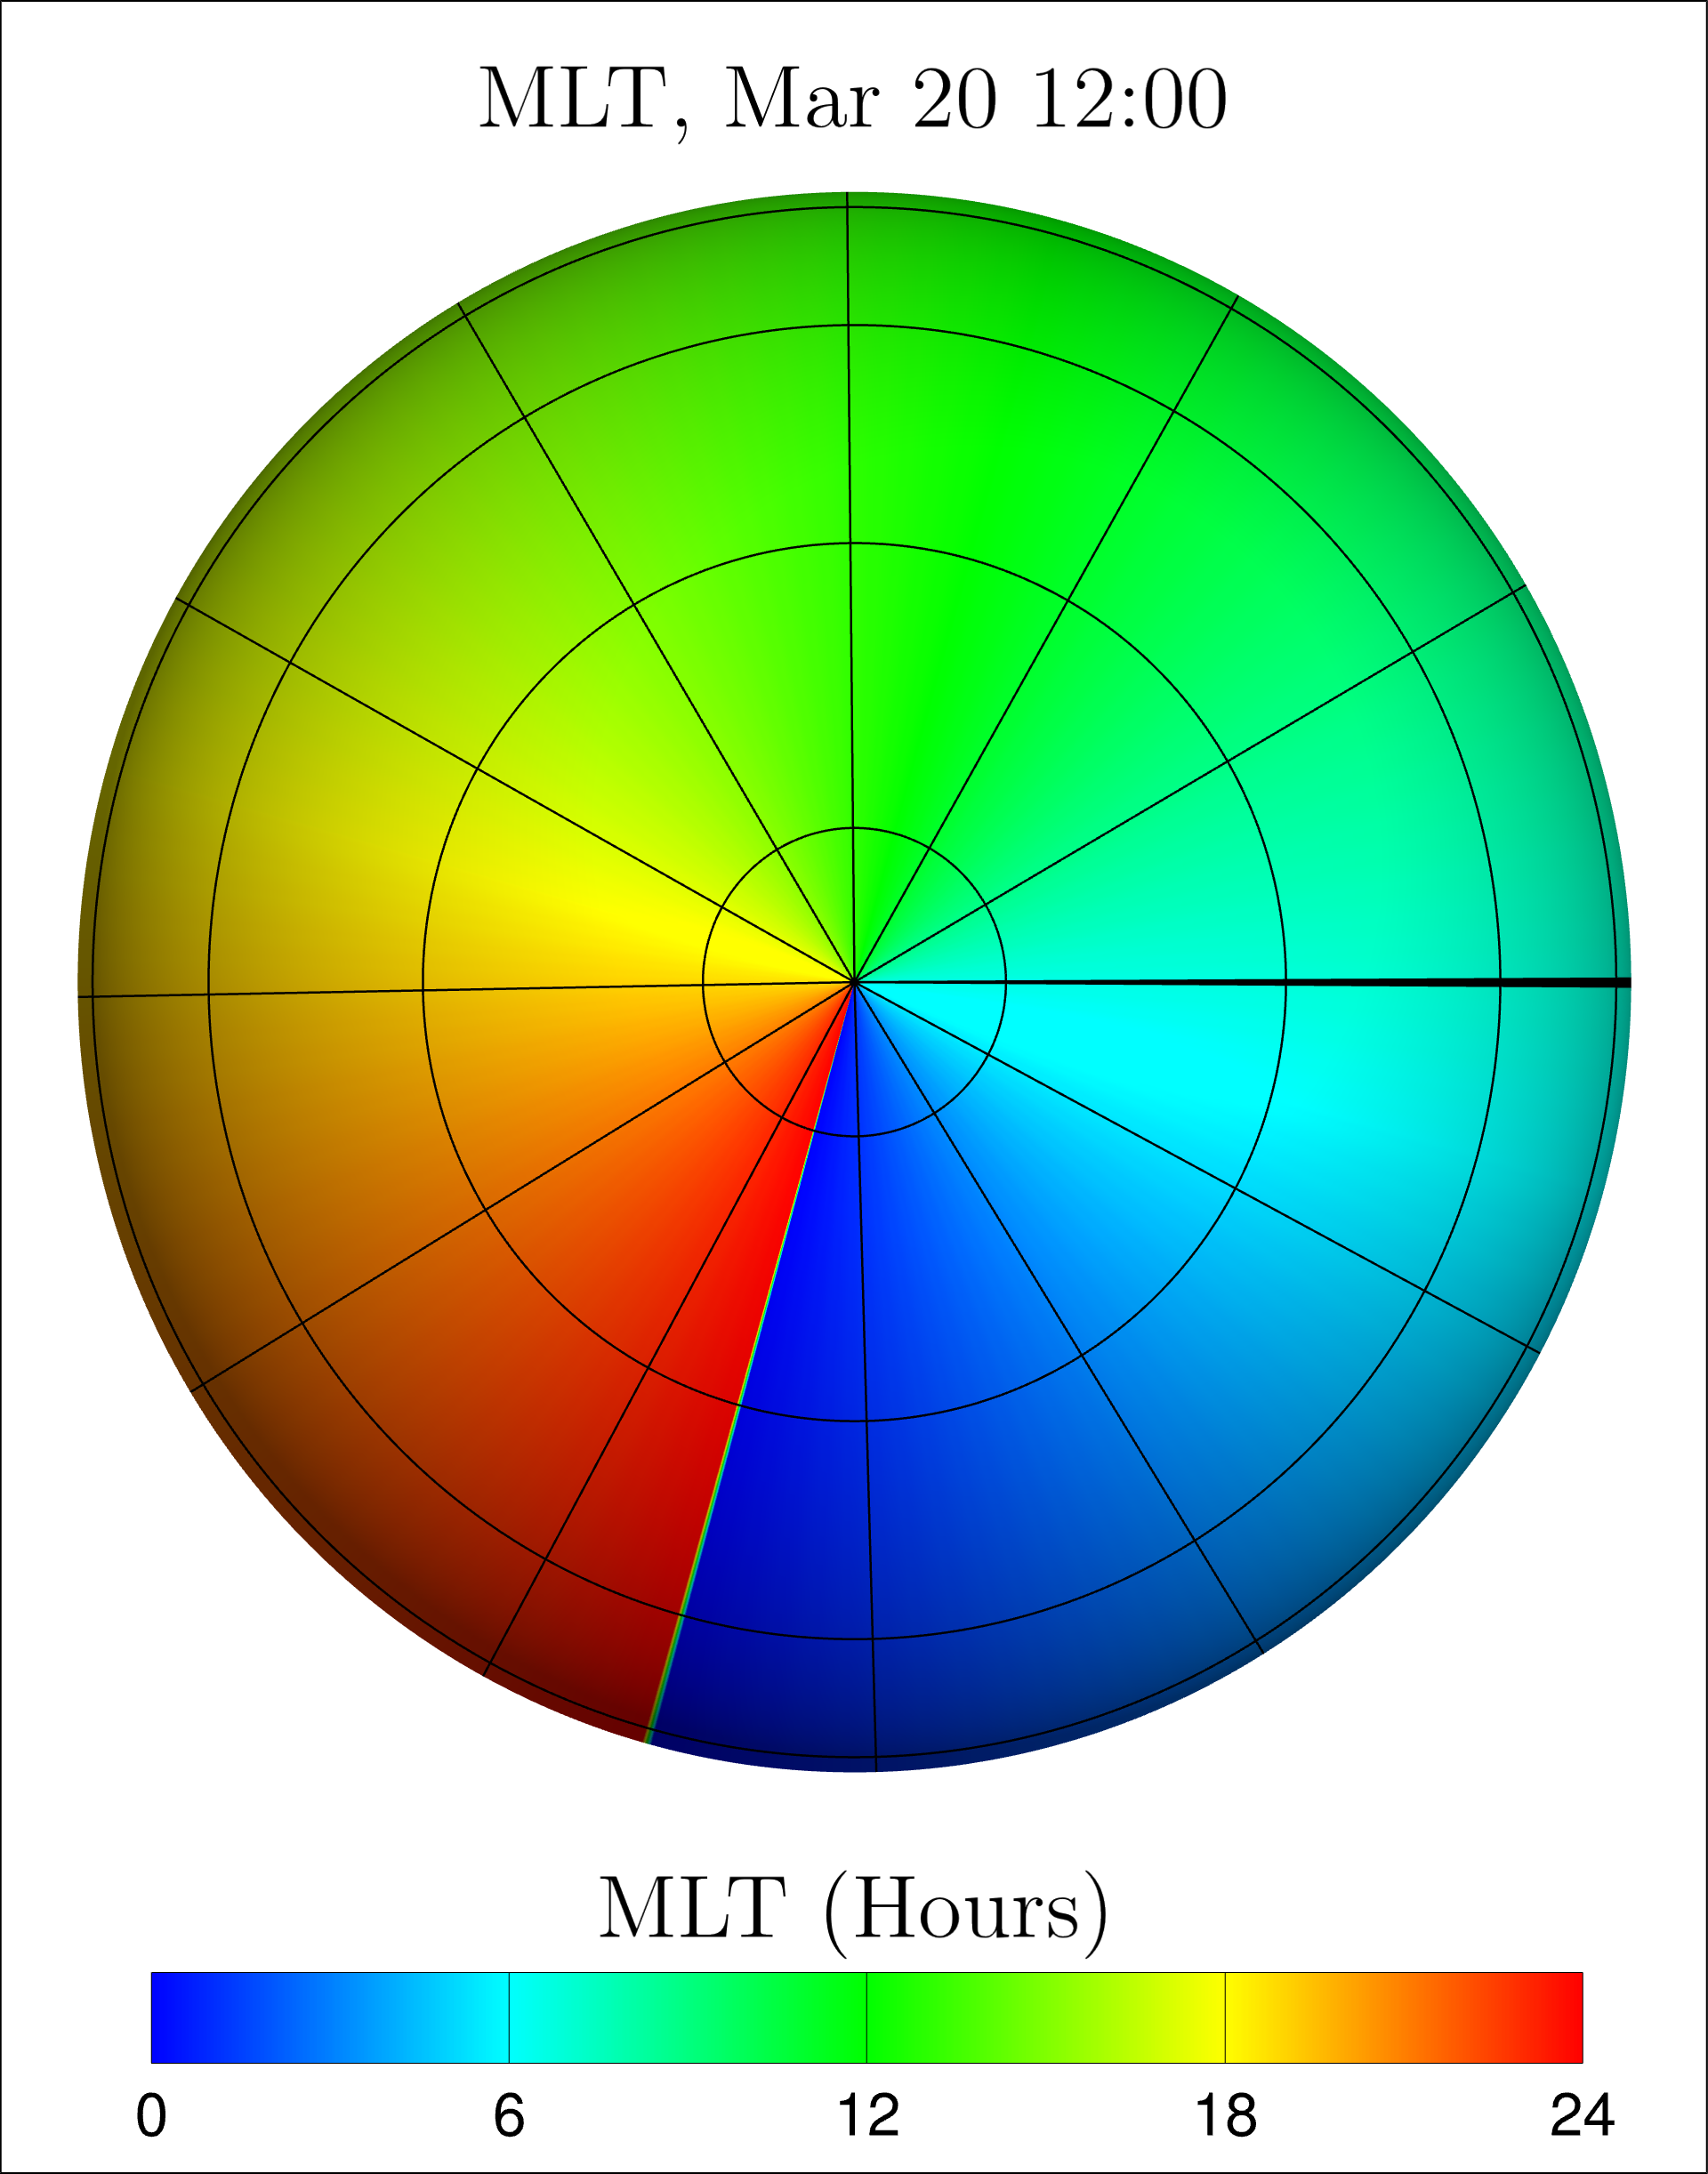
\includegraphics[width=0.4\textwidth]{figures/mltAlignment.png}
	\caption{Magnetic local time (MLT) in hours mapped onto the ionospheric sphere at equinox (Mar 20, 12:00).}
	\label{fig:mltAlignment}
\end{figure}
\section{Parallel Conductivity}
One large component that has been deferred from discussion so far is the parallel conductivity ($\sigz$). The parallel conductivity measures the conductivity along the magnetic field lines of the ionosphere. This is not widely available through empirical models as the Hall and Pedersen conductivity are. Therefore, the choice was made for the first iteration of this application to use the value $\sigz=1000\textrm{mhos}$. This serves as a reasonable stand in for the parallel conductivity due to the higher order of magnitude it exhibits~\citep{ionospheric_ridley_2003} relative to the Hall and Pederson conductivities. Future work is planned to investigate the feasibility of ionosphere models such as NRLMSIS~\citep{nrlmsis_emmert_2020} and IRI~\citep{international_bilitza_2022} to provide ion, electron and neutral densities. These could theoretically be used with the collision model in Equation~\ref{eq:physical_conduct} to derive all three conductivities from a first-principles approach. Further testing is required to verify the validity of this approach. This approach would allow for a value to be computed for the parallel conductivity, removing the need for the constant approximation.
